\documentclass{standalone}
\usepackage{tikz}
\begin{document}
\scriptsize
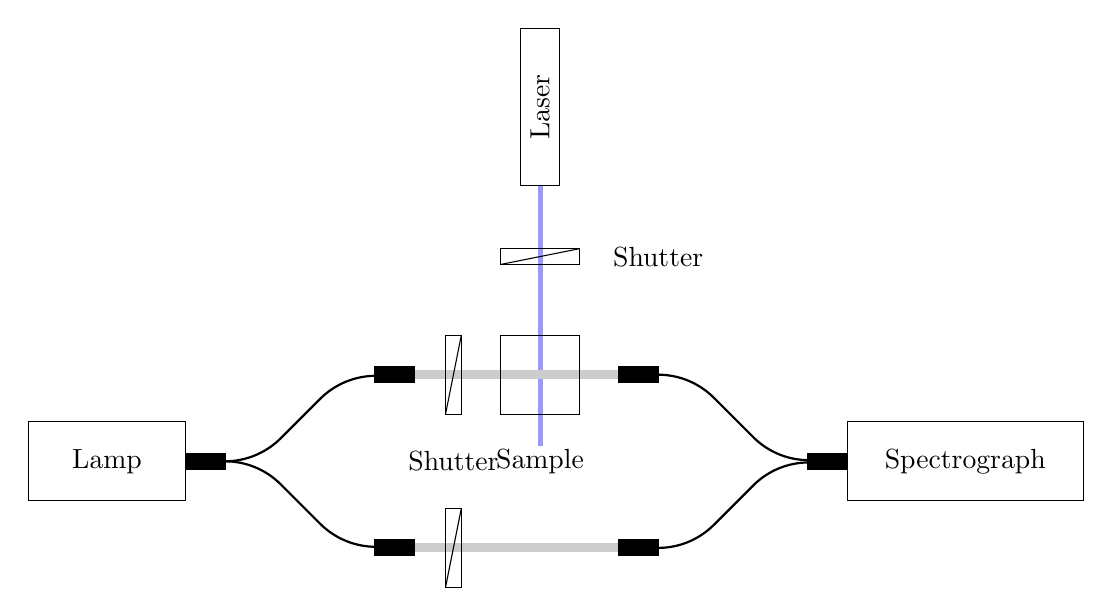
\begin{tikzpicture}
  \draw[draw=blue!40,fill=blue!40] (6.475,4) rectangle (6.525,0.7);
  \draw[draw=black!20,fill=black!20] (4.9,1.55) rectangle (7.5,1.65);
  \draw[draw=black!20,fill=black!20] (4.9,-0.65) rectangle (7.5,-0.55);
  %
  \draw (0,0) rectangle ++(2,1);
  \draw (1,0.5) node {Lamp};
  \draw[fill] (2,0.4) rectangle ++(0.5,0.2);
  \draw[thick] (2.5,0.5) arc (-90:-45:1) -- ++(0.5,0.5) arc (135:90:1);
  \draw[fill] (4.4,1.5) rectangle ++(0.5,0.2);
  %
  \draw (6,1.1) rectangle ++(1,1);
  \draw (6.5,0.5) node {Sample};
  %
  \draw (5.3,1.1) rectangle ++(0.2,1);
  \draw (5.3,1.1) -- ++(0.2,1);
  \draw (5.4,0.5) node {Shutter};
  %
  \draw[fill] (7.5,1.5) rectangle ++(0.5,0.2);
  \draw[thick] (8,1.6) arc (90:45:1) -- ++(0.5,-0.5) arc (225:270:1);
  \draw[fill] (9.9,0.4) rectangle ++(0.5,0.2);
  %
  \draw (10.4,0) rectangle ++(3,1);
  \draw (11.9,0.5) node {Spectrograph};
  %
  \draw[thick] (2.5,0.5) arc (90:45:1) -- ++(0.5,-0.5) arc (225:270:1);
  \draw[fill] (4.4,-0.7) rectangle ++(0.5,0.2);
  %
  \draw (5.3,-1.1) rectangle ++(0.2,1);
  \draw (5.3,-1.1) -- ++(0.2,1);
  %
  \draw[fill] (7.5,-0.7) rectangle ++(0.5,0.2);
  \draw[thick] (8,-0.6) arc (-90:-45:1) -- ++(0.5,0.5) arc (135:90:1);
  %
  \draw (6.25,4) rectangle ++(0.5,2);
  \draw (6.5,5) node [rotate=90] {Laser};
  %
  \draw (6,3) rectangle ++(1,0.2);
  \draw (6,3) -- ++(1,0.2);
  \draw (8,3.1) node {Shutter};
  %
\end{tikzpicture}
\end{document}
